\documentclass{article}
\usepackage[slovak]{babel}
\usepackage[utf8]{inputenc}
\usepackage{hyperref}
\hypersetup{colorlinks=true, linkcolor=black, urlcolor=blue}
\usepackage{indentfirst}
\usepackage[left=2.5cm,text={16cm, 22cm},top=3.5cm]{geometry}
\usepackage{graphicx}

\begin{document}
    \begin{titlepage}
        \begin{center}
            \textsc{\Huge Vysoké učení technické v~Brně\\
            		\huge Fakulta informačních technologií\\}
            \vspace{\stretch{0.382}}
            {\LARGE ISA - Síťové aplikace a~správa sítí\\}\vspace{2em}
            {\Large dokumentácia k 2.variante projektu\\}\vspace{2em}
            \Huge dns-export\\
            \vspace{\stretch{0.618}}
        \end{center}
        {\Large \today \hfill Tomáš Nereča}\vspace{-2em}
    \end{titlepage}

    \tableofcontents
        \thispagestyle{empty}
        \newpage
        \setcounter{page}{1}
    \newpage
    
    \section{Úvod}

        \textbf{dns-export} je aplikácia na spracovávanie dát protokolu \emph{DNS (Domain Name System)}.
        Aplikácia teda musí vedieť identifikovať a spracovať \emph{paket} daného protokolu.
        Jednotlivé pakety môže buď čerpať z \emph{pcap} súboru alebo odchytávať v reálnom čase
        zo sieťového rozhrania.

        Zo spracovaných dát vytvára štatistiky, ktoré v časovom intervale posiela protokolom \emph{Syslog}
        na centrálny logovací server alebo jednoducho vypisuje na štandardný výstup. Zbierané štatistiky sú:\\
        \texttt{domain-name rr-type rr-answer a count}.
    
    \section{Návrh aplikácie}

        \subsection{Objektový návrh}
        Svoju aplikáciu som sa rozhodol naprogramovať objektovo. Dodržiaval som štruktúru jedna \emph{trieda}
        na jeden zdrojový súbor. Každá trieda má svoju významom vyhradenú funkciu. 

        \subsection{Spracovanie paketov}
        Aplikácia spracuje vstupné argumenty a po ich validácii sa buď spustí spracovanie pcap súboru, alebo odchytávanie
        paketov zo sieťového rozhrania. Pre každý spracovávaný paket sa vytvorí objekt držiaci dáta paketu.

        V tomto objekte sa najprv spracujú jednotlivé hlavičky paketu. Ak sa zistí, že paket obsahuje odpovede na DNS otázky,
        Vytvorí sa pre každú odpoveď objekt, ktorý tieto odpovede spracováva.

        \subsection{Ukladanie štatistík}
        Po úspešnom spracovaní odpovedí sa každá odpoveď pridá do objektu, ktorý obsahuje kolekciu všetkých nazbieraných štatistík.
        Pomocou metódy sa zistí, či sa daná štatistická informácia v objekte už nachádza a v tom prípade sa len inkrementuje počítadlo.
        
        \subsection{Odosielanie a výpis štatistík}
        Po prečítaní z pcap súboru sa štatistiky uložené v objekte odošlú na server ak je zadaný alebo vypíšu na štandardný výstup.
        V prípade živého odchytávania sa pred jeho spustením vytvorí separátne vlákno, ktoré bude v zadanom časovom intervale
        odosielať všetky doposiaľ nazbierané štatistiky. Okrem toho bude aplikácia pri odchytení signálu \textbf{SIGUSR1} volať funkciu
        na výpis štatistík na štandardný výstup.
        
    \newpage

    \section{Implementácia}
    
        \subsection{DnsExport.cpp}
        Po spustení aplikácie je vytvorený objekt tejto triedy a zavolaná funkcia \textbf{Main()}. Nastaví sa odchýtavanie signálov
        a na základne vstupných argumentov načítaných pomocou vstavanej funkcie \textbf{getopt()}\footnote{http://man7.org/linux/man-pages/man3/getopt.3.html} sa rozhodne, či sa spustí funkcia
        \textbf{sniffInterface()} alebo \textbf{sniffFile()}. 
        
        V prvom prípade sa pred započatím odchytávania spustí funkcia \textbf{sendingLoop()},
        ktorá sa v separátnom vlákne stará o pravidelné odosielanie na Syslog server. Pre odoslanie volá funkcia \textbf{sendStats()}, ktorá si volá
        pomocné funkcie na vytvorenie správ ako napr.: \textbf{getMessages()} alebo \textbf{getFormattedTime()} a následne \emph{UDP} protokolom 
        odosiela správy. Správa nie je dlhšia ako 1 kB a jednotlivé štatistiky sú oddelené znakom $\vert$.

        V druhom prípade ak nebol zadaný Syslog server, je po prečítaní súboru zavolaná funkcia \textbf{getMessages()}, ktorá štatistiky vypíše
        na štandardný výstup a aplikácia končí. Rovnaká funkcia je volaná aj pri prijatí signálu \textbf{SIGUSR1}.

        O všetky akcie ohľadom odchytávania paketov sa stará knižnica \textbf{libpcap}\footnote{https://www.tcpdump.org/pcap.html}. Pre každý paket
        je volaná \emph{callback} funkcia \textbf{pcapHandler()}. Tam je vytvorený objekt triedy \textbf{DnsPacket} a zavolaná funkcia \textbf{Parse()}.

        Ak boli v pakete nájdené validné DNS odpovede - \emph{answers}, je zavolaná funkcia \textbf{addRecords()}, ktorá do globálnej premennej \textbf{recordList} pridá nový
        objekt triedy \textbf{DnsRecord}, ak sa daná štatistika v liste ešte nenachádza, alebo len zvýši počítadlo u nájdenej štatistiky.

        \subsection{DnsPacket.cpp}
        Vo funkcii \textbf{Parse()} je najprv zavolaná funkcia \textbf{getTransProt()}. Tá parsuje \emph{ethernet} hlavičku (podporované typy sú IPv4 a IPv6)
        a následne zistí transportný protokol (podporované typy sú UDP a TCP) a skočí na pozíciu, kde by sa mala nachádzať DNS hlavička.

        Parsovanie DNS hlavičky začína vo funkcii \textbf{dnsParse()}. Tam prebehnú validácie, či ide skutočne o DNS paket. \emph{query} pakety sú
        ignorované, aplikácia pracuje len s answers. Ak sú nájdené answers, je zavolaná funkcia \textbf{parseRRSet()}, kde je hneď na začiatku zavolaná funkcia \textbf{skipQuestion()}, ktorá
        skočí na pozíciu prvej answer.

        Pre každú answer je vytvorený objekt triedy \textbf{DnsRR}, ktorý spracuje dáta a nastaví pozíciu na ďalšiu answer. Ak boli získané nejaké dáta, objekt je uložený do listu
        \textbf{Answers}.

        \newpage

        \subsection{DnsRR.cpp}
        Každá answer začína \emph{domain-name}, ktorý je získaný funkciou \textbf{readDomainName()}. Ak sa podarí získať domain-name, nasleduje získanie \emph{rr-type} a dĺžky dát.
        Vo funkcii \textbf{applyParser()} je \textbf{switch}, v ktorom sa na základe typu záznamu rozhodne ktorý z parserov\footnote{Konkrétnejší popis jednotlivých parserov je v komentároch v zdrojovom kóde. 
        Veľmi špecifický je záznam typu \texttt{SPF}. V súčasnosti sa posielajú iba záznamy typu \texttt{TXT} ktoré sa dajú na základe určitých pravidiel označiť ako \texttt{SPF}. Toto aplikácia nezisťuje
        a každý \texttt{TXT} záznam označí typom \texttt{TXT}. Keby náhodou prišiel záznam typu \texttt{SPF}, je parsovaný rovnako ako klasický \texttt{TXT} záznam.} pre dáta použiť. Okrem toho sa typ uloží ako \emph{string}
        hodnota pre jednoduchšie ukladanie štatistík. Ak sa podarilo získať dáta, je vrátená pozícia za odpoveďou a aplikácia pokračuje parsovaním ďalšej answer.

        \subsection{Helpers.cpp}
        Táto trieda obsahuje makrá pre logovanie \textbf{LOGGING} a ukončovanie aplikácie ak nastane problém \textbf{ERR\_RET}.

        Funkcia \textbf{ToHex()} prevedie netlačiteľný znak do hexadecimálneho tvaru, napr.: \texttt{0x01}. Je používaná ak sa napríklad v domain-name alebo \texttt{TXT}
        zázname objaví netlačiteľný znak.

        Funkcia \textbf{Base64Encode()} je využívaná parseroch pre záznamy typu \texttt{DNSKEY, DS a RRSIG}. Kóduje bajtové pole ako base64 string, ktorý sa zobrazí v štatistikách.
        Funkcia je dostupná na githube\footnote{https://github.com/ReneNyffenegger/cpp-base64/blob/master/base64.cpp} pod \emph{Zlib} licenciou. 

        \newpage

    \section{Zaujímavé časti kódu}
        \subsection{LINUX\_SLL datalink}
        Pri odchytávaní na všetkých rozhraniach (interface=any), nemajú pakety ethernet hlavičku ale tzv. \emph{"linux-coocked header"}.
        To sa dá zistiť pomocou funkcie \textbf{pcap\_datalink()}. Ak ide o \texttt{LINUX\_SLL\_DATALINK}, hlavička je parsovaná iným spôsobom ako ethernet:\\\\
        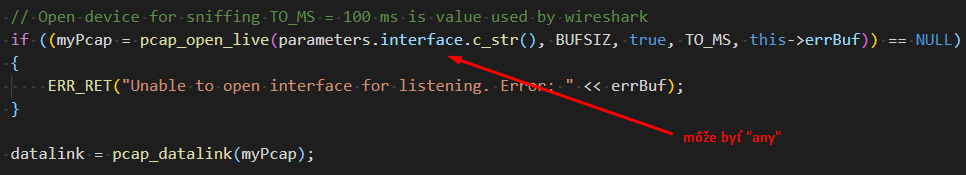
\includegraphics[scale=0.6]{datalink.png}\\\\
        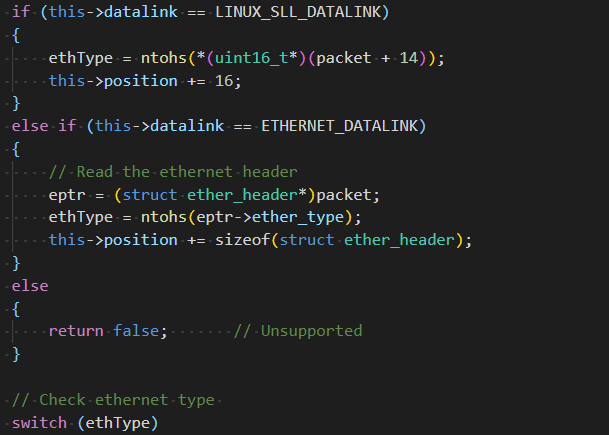
\includegraphics[scale=0.6]{ethernet.png}

        \newpage

        \subsection{Odosielanie na Syslog}
        Pri spustení vlákna na odosielanie sa najprv vyčká 20 ms a až potom sa spustí cyklus na odosielanie. Pretože aplikácia využíva parameter \textbf{to\_ms}
        vo funkcii \textbf{pcap\_open\_live()}, chceme aby sa stihli vytvoriť všetky štatistiky pred odoslaním. Kód je inšpirovaný vláknom na stránke
        cplusplus.com\footnote{http://www.cplusplus.com/forum/beginner/91449/}.:\\\\
        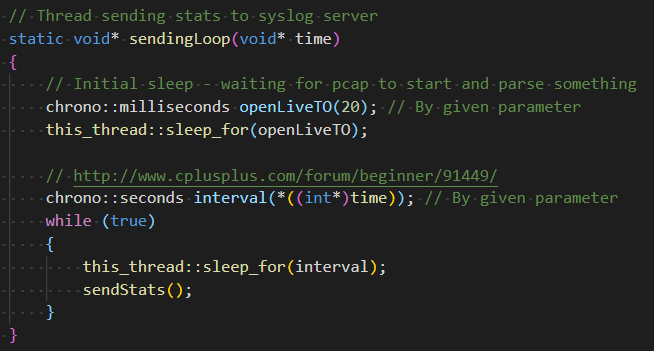
\includegraphics[scale=0.6]{loop.png}
        

        \subsection{Pole "hostname" v Syslog správe}
        RFC 5424\footnote{https://tools.ietf.org/html/rfc5424} špecifikuje prioritu. Aplikácia nepredpokladá existenciu FQDN ani statickú IP adresu, preto
        sa najprv pokúsi získať hostname a až v prípade neúspechu ip adresu.:\\\\
        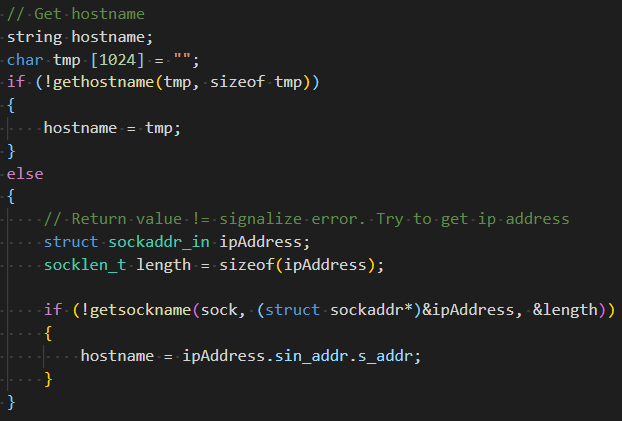
\includegraphics[scale=0.6]{hostname.png}

        \newpage

        \subsection{Získanie aktuálneho timestampu}
        Syslog správa potrebuje timestamp v špecifickom tvare. Kód je inšpirovaný vláknom na stránke
        codereview.stackexchange.com\footnote{https://codereview.stackexchange.com/questions/11921/getting-current-time-with-milliseconds}.:\\\\
        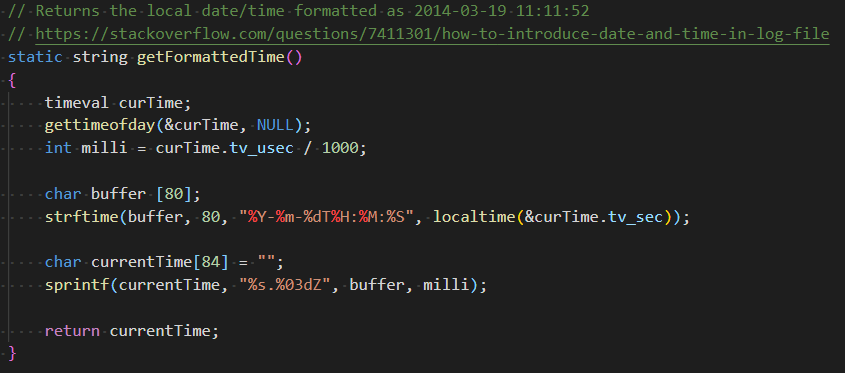
\includegraphics[scale=0.6]{timestamp.png}

        \newpage

        \subsection{Vytvorenie správ na odoslanie}
        Aplikácia vytvára správy s dĺžkou nepresahujúcou 1KB. Na Syslog server je v jednej správe posielaných viac štatistík oddelených znakom \texttt{|} .:\\\\
        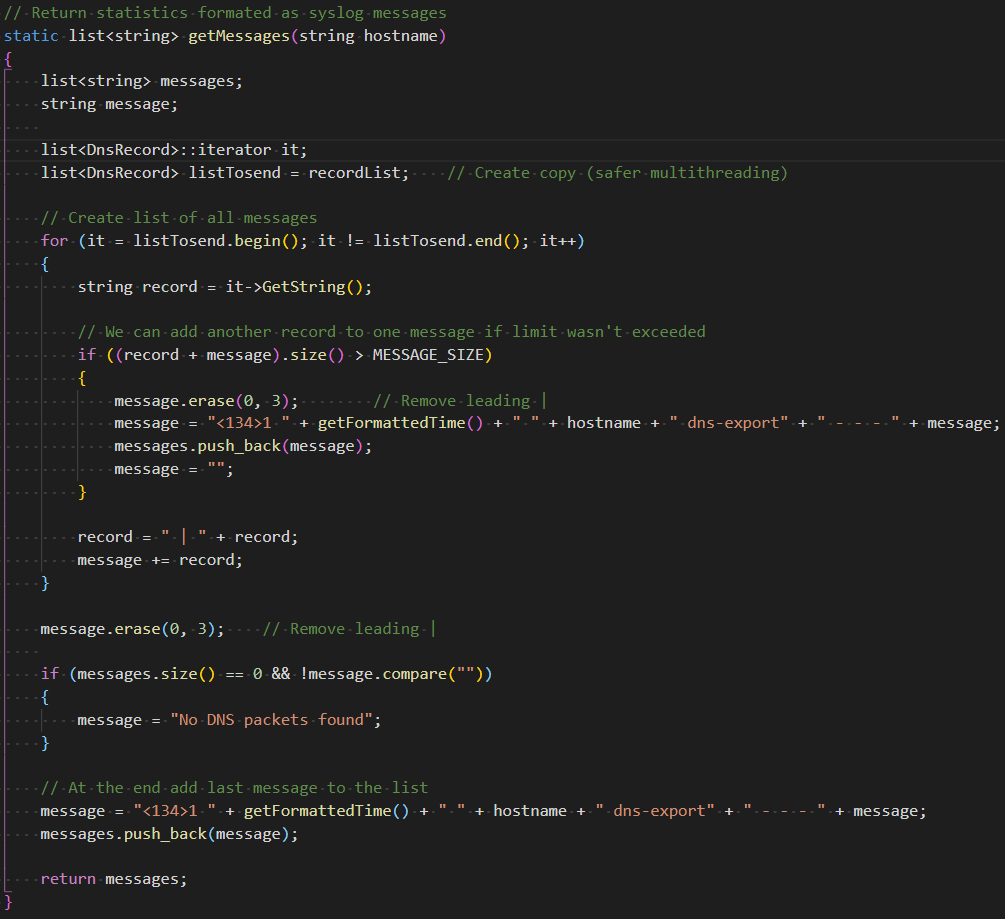
\includegraphics[scale=0.6]{messages.png}

        \newpage
        
    \section{Použitie}
        \subsection{Čítanie pcap súboru}
        \noindent
        Aplikácia sa spúšťa s argumentmi \textbf{-r} a \textbf{-s}:\\\\
        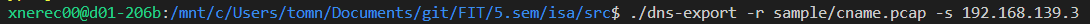
\includegraphics[scale=0.6]{r1.png}
        V tomto prípade sa na \textbf{stdout} nič nevypíše, štatistiky sú odoslané na Syslog server, napr.:\\\\
        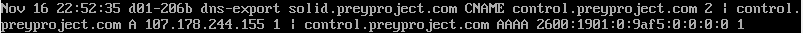
\includegraphics[scale=0.6]{r2.png}\\\\
        V prípade, že nie je zadaný Syslog server sa štatistiky vypíšu na \textbf{stdout}:\\\\
        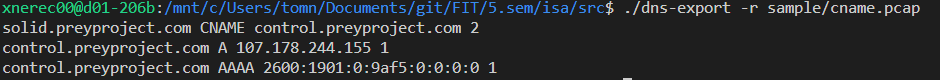
\includegraphics[scale=0.6]{r3.png}

        \subsection{Odchytávanie na rozhraní}
        \noindent
        Aplikácia sa spúšťa s argumentmi \textbf{-i}, \textbf{-s} a \textbf{-t}:\\\\
        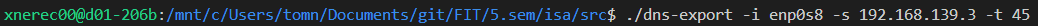
\includegraphics[scale=0.6]{i1.png}
        V tomto prípade budú štatistiky odosielané na Syslog server každých 45 sekúnd. Ak nie je zadaný argument \textbf{-t},
        štatistiky sú odosielané každých 60 sekúnd. Ak nie je zadaný argument \textbf{-s}, štatistiky sa neodosielajú.

        \subsection{Zaslanie signálu SIGUSR1}
        \noindent
        Pri odchytávaní na rozhraní sa štatistiky vypíšu na \textbf{stdout} pri zaslaní signálu \texttt{SIGUSR1}:\\\\
        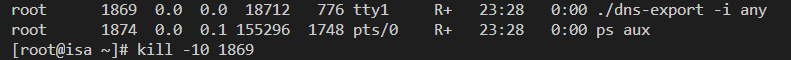
\includegraphics[scale=0.6]{i2.png}\\\\
        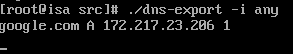
\includegraphics[scale=0.6]{i3.png}
    
    \newpage
    \section{Prehľad naštudovanej literatúry}
        \noindent
        Práca s knižnicou libpcap a parsovanie ethernetovej hlavičky a transportných protokolov - príklady
        k predmetu ISA (\texttt{sniff.c}, \texttt{read-pcap.c}) a rôzne voľne dostupné zdroje na internete.\\\\
        Syslog protokol - prednáška \texttt{isa-logovani.pdf}\\ 
        Parsovanie DNS hlavičky a jednotlivých typov záznamov - \texttt{RFC 1035}\\
        Parsovanie záznamov pre DNSSEC - \texttt{RFC 4034}\\
        Parsovanie hlavičky pri \texttt{LINKTYPE\_LINUX\_SLL} - \texttt{tcpdump.org}\\
        Špecifickost SPF záznamu - \texttt{support.dnsimple.com/}
    
    \section{Literatúra}
    \noindent
    \url{https://tools.ietf.org/html/rfc1035}\\
    \url{https://www.ietf.org/rfc/rfc4034.txt}\\
    \url{http://www.tcpdump.org/linktypes/LINKTYPE_LINUX_SLL.html}\\
    \url{https://support.dnsimple.com/articles/spf-record/}\\
    \url{https://en.wikipedia.org/wiki/List_of_DNS_record_types}\\
    \url{https://solarianprogrammer.com/2011/12/16/cpp-11-thread-tutorial/}\\
    \url{https://www.rhyous.com/2011/11/13/how-to-read-a-pcap-file-from-wireshark-with-c/}\\
    \url{https://www.tcpdump.org/pcap.html}\\
    \url{https://www.tcpdump.org/manpages/pcap_open_live.3pcap.html}\\

\end{document}